\documentclass[conference]{IEEEtran}
\IEEEoverridecommandlockouts
\usepackage{cite}
\usepackage{graphicx}
\usepackage{amsmath}
\usepackage{array}
\usepackage{booktabs}
\usepackage{siunitx}
\usepackage{xcolor}
\usepackage[hidelinks]{hyperref}
\usepackage{url}
\usepackage{tikz}
\usetikzlibrary{arrows.meta,positioning,shapes.geometric,shapes.misc,calc,matrix,fit}
\usepackage{enumitem}
\usepackage{listings}
\usepackage{textcomp}
\usepackage{tabularx}
\usepackage{placeins}
\usepackage{dblfloatfix}
\setlength{\textfloatsep}{8pt}
\setlength{\floatsep}{6pt}
\setlength{\intextsep}{6pt}
\renewcommand{\arraystretch}{1.15}
\setlength{\tabcolsep}{4.5pt}

\lstdefinestyle{sslgcode}{
  basicstyle=\ttfamily\footnotesize,
  columns=fullflexible,
  keepspaces=true,
  breaklines=true,
  frame=single,
  framerule=0.3pt,
  rulecolor=\color{black},
  showstringspaces=false
}

% Framed figure helpers: keep a consistent border and a consistent outer width.
\newcommand{\FrameBoxCol}[1]{%
  \begingroup
  \setlength{\fboxsep}{1pt}%
  \setlength{\fboxrule}{0.4pt}%
  \fbox{%
    \begin{minipage}{\dimexpr\columnwidth-2\fboxsep-2\fboxrule\relax}%
      \centering
      #1%
    \end{minipage}%
  }%
  \endgroup
}
\newcommand{\FrameBoxText}[1]{%
  \begingroup
  \setlength{\fboxsep}{1pt}%
  \setlength{\fboxrule}{0.4pt}%
  \fbox{%
    \begin{minipage}{\dimexpr\textwidth-2\fboxsep-2\fboxrule\relax}%
      \centering
      #1%
    \end{minipage}%
  }%
  \endgroup
}

% Fully clickable cross-references (click anywhere on "Fig. X" / "Table X").
\newcommand{\FigLink}[1]{\hyperref[#1]{Fig.~\ref*{#1}}}
\newcommand{\TabLink}[1]{\hyperref[#1]{Table~\ref*{#1}}}
\newcommand{\LstLink}[1]{\hyperref[#1]{Listing~\ref*{#1}}}

% Component thumbnail helper: consistent size across tables.
\newcommand{\CompThumb}[2]{%
  \IfFileExists{#1}{%
    \includegraphics[width=0.38\columnwidth,height=0.18\textheight,keepaspectratio]{#1}%
  }{%
    \fbox{\parbox[c][0.18\textheight][c]{0.38\columnwidth}{\centering \scriptsize #2\\\texttt{\detokenize{#1}}}}%
  }%
}

% Component full-view helper: framed, column-width, and height-tunable.
% Usage: \CompFull[<maxheight>]{<filename>}{<fallback label>}
\newcommand{\CompFull}[3][0.24\textheight]{%
  \IfFileExists{#2}{%
    \FrameBoxCol{\includegraphics[width=\linewidth,height=#1,keepaspectratio]{#2}}%
  }{%
    \FrameBoxCol{\parbox[c][#1][c]{\linewidth}{\centering \scriptsize #3\\\texttt{\detokenize{#2}}}}%
  }%
}

% --------- Team / Title-Page Metadata (edit these) ---------
\newcommand{\ProjectTitle}{Smart Sign Language Gloves (SSLG)}
\newcommand{\PaperTitle}{Smart Sign Language Gloves: A Real-Time ISL-to-Speech Translation System Using Hall Effect Sensors and Machine Learning}
\newcommand{\InstituteName}{Vidyavardhini's College Of Engineering \& Technology, Vasai Road}
\newcommand{\DeptName}{Department of Electronics and Communication Engineering}
\newcommand{\TeamMemberA}{Kushagra Naresh Joshi}
\newcommand{\TeamMemberB}{Afroz Abdul Inamdar}
\newcommand{\TeamMemberC}{Sakshi Rajendra Jagdale}
\newcommand{\TeamMemberD}{Ramzan Badruduja Khan}
\newcommand{\GuideName}{Project Guide: Prof. Shaista Khan}
\newcommand{\SubmissionDate}{March 2026}

\title{\PaperTitle}
\author{
    \IEEEauthorblockN{\TeamMemberA, \TeamMemberB, \TeamMemberC, \TeamMemberD}
    \IEEEauthorblockA{\DeptName\\
    \InstituteName\\
    Email: \{name1,name2,name3,name4\}@xyz.edu}
}

\begin{document}

% Page numbers in the footer, starting from the title page.
\pagenumbering{arabic}
\pagestyle{plain}
\raggedbottom

\begin{titlepage}
    \thispagestyle{plain}
    \centering
    \vspace*{0.8in}
    % College logo (ensure vect.png exists in the same folder as main.tex)
    \IfFileExists{vect.png}{
\includegraphics[width=0.22\textwidth]{vect.png}\par}{}
    \vspace{0.15in}
    {\Large \textbf{\InstituteName}\par}
    \vspace{0.08in}
    {\large \textbf{\DeptName}\par}
    \vspace{0.35in}
    {\Large \textbf{\ProjectTitle}\par}
    \vspace{0.2in}
    {\large \textbf{Technical Paper (IEEE-Style Draft)}\par}
    \vspace{0.35in}
    {\Large \textbf{\PaperTitle}\par}
    \vspace{0.45in}

    {\large \textbf{Team Members}\par}
    \vspace{0.1in}
    {\large \TeamMemberA\par}
    {\large \TeamMemberB\par}
    {\large \TeamMemberC\par}
    {\large \TeamMemberD\par}
    \vspace{0.35in}

    {\large \textbf{\GuideName}\par}
    \vfill
    {\large \SubmissionDate\par}
\end{titlepage}

% Intentionally blank page (for printing)
\clearpage
\thispagestyle{empty}
\null
\newpage

\maketitle
\thispagestyle{plain}

\begin{abstract}
Smart Sign Language Gloves (SSLG) aim to reduce communication barriers by translating Indian Sign Language (ISL) hand gestures into text and speech. The glove uses hall effect sensors and fingertip magnets to capture finger motion, an ATmega328P to sample and frame sensor data, and an ESP8266 link to send data to a Python Flask backend. The backend supports data collection, labeling, model training, and inference through a simple web interface. This paper describes the system design and implementation and presents an evaluation plan for accuracy and latency. Since full end-to-end testing is still in progress, expected performance ranges are reported and a clear format is provided for recording final measured results.
\end{abstract}

\begin{IEEEkeywords}
sign language recognition, hall effect sensors, machine learning, ISL, wearable computing, gesture classification
\end{IEEEkeywords}

\section{Introduction}
People with hearing and speech impairments often rely on sign language, but most people around them do not understand it. A practical ISL translator should be portable, low-cost, and fast enough to respond in real time. Camera-based systems can work well, but they often depend on good lighting and clear framing and can fail with occlusion\cite{mitra}. Wearable gloves avoid many camera issues, but flex sensors can be fragile and may drift over time. SSLG uses hall effect sensors and fingertip magnets to capture hand movement in a more durable way, and it uses a backend model to convert sensor patterns into an ISL label that can be displayed and spoken.

\subsection{Problem Formulation and Scope}
Many ISL translation systems either depend on cameras (higher cost and setup constraints) or use flex sensors (wear and drift). SSLG focuses on hall sensors and magnets to keep the glove simple, portable, and repeatable.

To keep the work manageable, we focus on:
\begin{itemize}[noitemsep]
    \item 20 commonly used ISL gestures for training and testing.
    \item Indoor laboratory testing with controlled conditions.
    \item Adult volunteer participants with repeatable sensor placement.
\end{itemize}

\section{Literature Review / Related Work}
\subsection{Systematic Search Strategy}
We reviewed recent work from IEEE Xplore, Scopus, and Google Scholar on sign/gesture recognition, wearable glove sensing, and practical deployment constraints (2018--2024).

\subsection{Critical Appraisal and Thematic Synthesis}
Prior work mainly falls into two groups: camera-based recognition and sensor-based gloves. Camera-based systems can recognize gestures without wearable hardware, but they often need stable lighting and clear framing and can fail with occlusion\cite{mitra}. Sensor gloves measure finger and hand motion directly and can work in many environments, but earlier designs that used flex sensors can degrade with repeated bending and show non-linear drift.

Gesture classification is time-dependent: even ``static'' signs include small movements and transitions that vary across people. Models that combine convolution layers (local patterns) with recurrent layers (sequence patterns) are commonly used. TensorFlow Lite is a practical choice for running trained models efficiently\cite{tensorflow}. SSLG follows this direction by using hall sensors for steadier inputs and by keeping the training and inference steps on the backend so the model can be updated as more data is collected.

\subsection{Identified Limitations in Prior Systems}
Many published demos do not fully discuss practical issues such as calibration time, long-term sensor changes, wireless packet loss, or the effort needed for labeling data. In real use, these details matter as much as the model choice. SSLG therefore puts emphasis on stable sensing and a clear data collection and labeling workflow.

\section{Proposed System / Methodology}
\subsection{System Overview}
SSLG is a wearable ISL-to-speech translator designed around two cooperating layers: (i) a glove-side sensing and sampling layer that captures hall sensor and IMU signals using an ATmega328P, and (ii) a backend software layer that performs labeling, dataset management, model training, and inference via a Flask server. This separation allows the recognition model to be improved over time without changing the glove hardware.

\subsection{Hardware Components}
This subsection lists the main hardware components used in SSLG in a fixed order. Each component is documented with (a) a short description, (b) a compact specification table, and (c) a full-view reference image.

\subsubsection{1) Microcontroller: ATmega328P, 16 MHz clock}
\textbf{a) Description:} The ATmega328P is the core controller of the glove. It samples five hall sensor channels using the 10-bit ADC, reads the MPU-6050 over I\textsuperscript{2}C, applies calibration/baseline subtraction, and frames UART packets for the ESP-01 uplink. The 16 MHz clock provides stable sampling intervals for consistent windowed features.\cite{atmega328p}

\textbf{b) Specification:} Shown in \TabLink{tab:atmega_specs}.
\begin{table}[!htbp]
    \centering
    \caption{ATmega328P Specifications}
    \label{tab:atmega_specs}
    \begin{tabularx}{\columnwidth}{@{}lX@{}}
        \toprule
        Parameter & Specification \\
        \midrule
        Architecture & 8-bit AVR RISC \\
        Clock speed & Up to 20 MHz (5 V) \\
        Flash / SRAM / EEPROM & 32 KB / 2 KB / 1 KB \\
        Supply voltage & 1.8 V to 5.5 V \\
        GPIO & 23 programmable I/O \\
        ADC & 10-bit, up to 8 channels \\
        Interfaces & USART, SPI, I\textsuperscript{2}C (TWI) \\
        Operating temp. & -40$^\circ$C to +85$^\circ$C \\
        \bottomrule
    \end{tabularx}
\end{table}

\textbf{c) Image:} Shown in \FigLink{fig:atmega_img}.
\begin{figure}[!htbp]
    \centering
    \CompFull[0.22\textheight]{comp_atmega328p.png}{ATmega328P image}
    \caption{ATmega328P microcontroller (reference image).}
    \label{fig:atmega_img}
\end{figure}
\FloatBarrier

\subsubsection{2) Programmer: FTDI FT232RL USB-to-UART}
\textbf{a) Description:} The FTDI FT232RL board is used to flash firmware and debug the serial data stream. It provides a stable USB-to-TTL UART interface compatible with the Arduino toolchain. During ESP-01 flashing, the ESP should be powered from the dedicated 3.3 V rail (not the FTDI 3.3 V pin) because Wi-Fi transmit bursts can exceed the FTDI board's regulator capability.\cite{ft232rl}

\textbf{b) Specification:} Shown in \TabLink{tab:ftdi_specs}.
\begin{table}[!htbp]
    \centering
    \caption{FTDI FT232RL Specifications}
    \label{tab:ftdi_specs}
    \begin{tabularx}{\columnwidth}{@{}lX@{}}
        \toprule
        Parameter & Specification \\
        \midrule
        USB standard & USB 2.0 full-speed (12 Mb/s) \\
        Voltage select & 3.3 V / 5 V selectable \\
        3.3 V rail output & $\sim$50 mA (board-dependent) \\
        Baud rate range & 300 bps to 3,000,000 bps \\
        Buffers & TX 256 bytes; RX 128 bytes \\
        Drivers & VCP drivers (Windows/macOS/Linux) \\
        \bottomrule
    \end{tabularx}
\end{table}

\textbf{c) Image:} Shown in \FigLink{fig:ftdi_img}.
\begin{figure}[!htbp]
    \centering
    \CompFull[0.20\textheight]{comp_ftdi.png}{FTDI FT232RL image}
    \caption{FTDI FT232RL USB-to-UART programmer (reference image).}
    \label{fig:ftdi_img}
\end{figure}
\FloatBarrier

\subsubsection{3) Charger: TP4056 Type-C single-cell charger module}
\textbf{a) Description:} The TP4056 module charges the single-cell 18650 battery from a USB-C supply using a CC/CV profile with charge termination. It provides a compact and low-complexity charging solution appropriate for portable wearables.\cite{tp4056}

\textbf{b) Specification:} Shown in \TabLink{tab:tp4056_specs}.
\begin{table}[!htbp]
    \centering
    \caption{TP4056 Specifications}
    \label{tab:tp4056_specs}
    \begin{tabularx}{\columnwidth}{@{}lX@{}}
        \toprule
        Parameter & Specification \\
        \midrule
        Input voltage ($V_{IN}$, max) & 8 V \\
        Charge current ($I_{CHG}$, max) & 1000 mA (programmable via $R_{PROG}$) \\
        Regulation voltage & 4.2 V $\pm$ 1.5\% \\
        Trickle threshold & 2.9 V \\
        Termination current & $0.1 \times I_{CHG}$ \\
        Standby current & $\sim$4 $\mu$A \\
        Operating temp. & -20$^\circ$C to +85$^\circ$C \\
        Topology & CC/CV linear charger \\
        \bottomrule
    \end{tabularx}
\end{table}

\textbf{c) Image:} Shown in \FigLink{fig:tp4056_img}.
\begin{figure}[!htbp]
    \centering
    \CompFull[0.19\textheight]{comp_tp4056.png}{TP4056 module image}
    \caption{TP4056 Type-C charger module (reference image).}
    \label{fig:tp4056_img}
\end{figure}
\FloatBarrier

\subsubsection{4) Battery: 18650 Li-ion, 3.7 V nominal}
\textbf{a) Description:} The 18650 Li-ion cell is the primary energy source for SSLG. It offers good energy density and is widely available. For safety, a protected cell or protection circuitry is recommended (overcharge, over-discharge, and short-circuit protection).\cite{battery18650}

\textbf{b) Specification:} Shown in \TabLink{tab:18650_specs}.
\begin{table}[!htbp]
    \centering
    \caption{18650 Cell Specifications}
    \label{tab:18650_specs}
    \begin{tabularx}{\columnwidth}{@{}lX@{}}
        \toprule
        Parameter & Specification \\
        \midrule
        Nominal voltage & 3.6 V / 3.7 V \\
        Full charge voltage & 4.2 V $\pm$ 50 mV \\
        Cutoff voltage & 2.5 V to 3.0 V \\
        Typical capacity & 1800 mAh to 3500 mAh \\
        Max discharge current & 2C to 10C (cell-dependent) \\
        Dimensions & 18.6 mm $\times$ 65.0 mm \\
        Cycle life & 300 to 500 cycles @ 80\% capacity \\
        Operating temp. & -20$^\circ$C to +60$^\circ$C (charge: 0$^\circ$C to 45$^\circ$C) \\
        \bottomrule
    \end{tabularx}
\end{table}

\textbf{c) Image:} Shown in \FigLink{fig:18650_img}.
\begin{figure}[!htbp]
    \centering
    \CompFull[0.19\textheight]{comp_battery_18650.png}{18650 battery image}
    \caption{18650 Li-ion battery cell (reference image).}
    \label{fig:18650_img}
\end{figure}
\FloatBarrier

\subsubsection{5) Boost Converter: MT3608, 33 uH inductor, 5 V rail}
\textbf{a) Description:} The MT3608 boost converter steps up the battery voltage to a 5 V rail used by the ATmega328P and the analog sensor front-end. Since it is a switching converter, ripple control is important; the design uses local decoupling and careful return paths to reduce noise coupling into ADC channels.\cite{mt3608}

\textbf{b) Specification:} Shown in \TabLink{tab:mt3608_specs}.
\begin{table}[!htbp]
    \centering
    \caption{MT3608 Specifications}
    \label{tab:mt3608_specs}
    \begin{tabularx}{\columnwidth}{@{}lX@{}}
        \toprule
        Parameter & Specification \\
        \midrule
        Input voltage ($V_{IN}$) & 2 V to 24 V \\
        Output voltage ($V_{OUT}$) & 5 V to 28 V (adjustable) \\
        Output current ($I_{OUT}$, max) & 2 A \\
        Switching frequency & 1.2 MHz (typ.) \\
        Efficiency & Up to 93\% \\
        Quiescent current & $\sim$1 mA (typ.) \\
        Operating temp. & -40$^\circ$C to +85$^\circ$C \\
        \bottomrule
    \end{tabularx}
\end{table}

\textbf{c) Image:} Shown in \FigLink{fig:mt3608_img}.
\begin{figure}[!htbp]
    \centering
    \CompFull[0.20\textheight]{comp_mt3608.png}{MT3608 module image}
    \caption{MT3608 boost module (reference image).}
    \label{fig:mt3608_img}
\end{figure}
\FloatBarrier

\subsubsection{6) Buck Converter: LM2596 switching buck, adjusted to 3.3 V rail}
\textbf{a) Description:} The LM2596 buck converter provides a regulated 3.3 V rail for the ESP-01 module. A switching buck is selected to reduce heat under high Wi-Fi burst currents. Output capacitance and a bulk+ceramic decoupling network are used near the ESP-01 to mitigate brownouts.\cite{lm2596}

\textbf{b) Specification:} Shown in \TabLink{tab:lm2596_specs}.
\begin{table}[!htbp]
    \centering
    \caption{LM2596 Specifications}
    \label{tab:lm2596_specs}
    \begin{tabularx}{\columnwidth}{@{}lX@{}}
        \toprule
        Parameter & Specification \\
        \midrule
        Input voltage ($V_{IN}$) & 4.5 V to 40 V \\
        Output voltage ($V_{OUT}$) & 1.23 V to 37 V (adj.) / fixed variants \\
        Output current ($I_{OUT}$) & 3 A (rated) \\
        Switching frequency & 150 kHz (fixed) \\
        Output accuracy & $\pm$4\% \\
        Efficiency & Up to 92\% \\
        Operating temp. & -40$^\circ$C to +125$^\circ$C \\
        \bottomrule
    \end{tabularx}
\end{table}

\textbf{c) Image:} Shown in \FigLink{fig:lm2596_img}.
\begin{figure}[!htbp]
    \centering
    \CompFull[0.21\textheight]{comp_lm2596.png}{LM2596 module image}
    \caption{LM2596 buck module (reference image).}
    \label{fig:lm2596_img}
\end{figure}
\FloatBarrier

\subsubsection{7) Wi-Fi Module: ESP-01 (ESP8266EX)}
\textbf{a) Description:} The ESP-01 (ESP8266EX) provides the wireless uplink. It bridges the UART stream coming from the ATmega328P to the backend Flask server over Wi-Fi using HTTP requests. It requires a stable 3.3 V rail because peak TX currents can be high.\cite{esp8266}

\textbf{b) Specification:} Shown in \TabLink{tab:esp_specs}.
\begin{table}[!htbp]
    \centering
    \caption{ESP-01 (ESP8266) Specifications}
    \label{tab:esp_specs}
    \begin{tabularx}{\columnwidth}{@{}lX@{}}
        \toprule
        Parameter & Specification \\
        \midrule
        Supply voltage & 3.0 V to 3.6 V (3.3 V nominal) \\
        Wi-Fi standard & IEEE 802.11 b/g/n (2.4 GHz) \\
        Peak TX current & $\sim$215 mA (burst) \\
        Modes & Station / Soft-AP / Station+AP \\
        UART & Default 115200 bps (typ., AT firmware) \\
        Security & WPA/WPA2-Personal \\
        Operating temp. & -40$^\circ$C to +125$^\circ$C \\
        \bottomrule
    \end{tabularx}
\end{table}

\textbf{c) Image:} Shown in \FigLink{fig:esp01_img}.
\begin{figure}[!htbp]
    \centering
    \CompFull[0.20\textheight]{comp_esp8266.png}{ESP-01 image}
    \caption{ESP-01 Wi-Fi module (reference image).}
    \label{fig:esp01_img}
\end{figure}
\FloatBarrier

\subsubsection{8) Finger Sensors: Hall sensors (SS49E linear / A3144 digital)}
\textbf{a) Description:} SSLG uses hall effect sensors placed near finger segments along with small fingertip magnets. Finger bending changes the magnet-to-sensor geometry and produces a characteristic multi-channel signature. Hall sensing is preferred over flex sensors for better reliability and reduced mechanical wear; the key remaining variability is magnet placement, which is handled through calibration and consistent mounting.\cite{ss49e}

\textbf{b) Specification:} Shown in \TabLink{tab:hall_specs}.
\begin{table}[!htbp]
    \centering
    \caption{Hall Sensor Specifications (Typical)}
    \label{tab:hall_specs}
    \begin{tabularx}{\columnwidth}{@{}lX@{}}
        \toprule
        Parameter & Specification \\
        \midrule
        Supply voltage ($V_{CC}$) & 3 V to 6 V (SS49E) / 4.5 V to 24 V (A3144) \\
        Output type & Analog ratiometric (SS49E) / open-collector (A3144) \\
        Sensitivity (SS49E) & $\sim$1.4 mV/Gauss (ratiometric) \\
        Response time & 2 $\mu$s (typ.) \\
        Operating temp. & -40$^\circ$C to +85$^\circ$C (typ.) \\
        Package & TO-92 (typ.) \\
        \bottomrule
    \end{tabularx}
\end{table}

\textbf{c) Image:} Shown in \FigLink{fig:hall_img}.
\begin{figure}[!htbp]
    \centering
    \CompFull[0.17\textheight]{comp_hall_sensor.png}{Hall sensor image}
    \caption{Hall effect sensor (reference image).}
    \label{fig:hall_img}
\end{figure}
\FloatBarrier

\subsubsection{9) IMU: MPU-6050, 6-axis (gyro + accelerometer)}
\textbf{a) Description:} The MPU-6050 provides hand/wrist motion context to complement finger sensing. The 3-axis accelerometer and 3-axis gyroscope make recognition more reliable for dynamic gestures and help separate signs with similar finger patterns.\cite{mpu6050}

\textbf{b) Specification:} Shown in \TabLink{tab:mpu_specs}.
\begin{table}[!htbp]
    \centering
    \caption{MPU-6050 Specifications}
    \label{tab:mpu_specs}
    \begin{tabularx}{\columnwidth}{@{}lX@{}}
        \toprule
        Parameter & Specification \\
        \midrule
        Supply voltage ($V_{DD}$) & 2.375 V to 3.46 V \\
        Gyro full-scale & $\pm$250 / $\pm$500 / $\pm$1000 / $\pm$2000 $^\circ$/s \\
        Accel full-scale & $\pm$2 / $\pm$4 / $\pm$8 / $\pm$16 g \\
        Resolution & 16-bit ADC \\
        Interface & I\textsuperscript{2}C (up to 400 kHz) \\
        FIFO buffer & 1024 bytes \\
        Operating temp. & -40$^\circ$C to +85$^\circ$C \\
        \bottomrule
    \end{tabularx}
\end{table}

\textbf{c) Image:} Shown in \FigLink{fig:mpu_img}.
\begin{figure}[!htbp]
    \centering
    \CompFull[0.20\textheight]{comp_mpu6050.png}{MPU6050 image}
    \caption{MPU-6050 IMU module (reference image).}
    \label{fig:mpu_img}
\end{figure}
\FloatBarrier

\subsection{Software / Algorithm}
The SSLG software stack consists of: (i) ATmega328P firmware for sampling and packet framing, (ii) ESP8266 Wi-Fi transport for uplink, and (iii) a Flask backend for data ingestion, labeling, model training, and inference. The main workflow is shown in Fig.~\ref{fig:mlflow}, and example code is provided in Listings~\ref{lst:flask_ingest}--\ref{lst:firmware_pack}.

\subsubsection{Communication Protocol}
The ATmega328P transmits sensor samples to the ESP-01 over UART (typical baud rate: 115200 bps). The ESP-01 forwards these frames to the Flask backend using HTTP requests. A lightweight acknowledgment mechanism (server response codes) can be used to detect packet loss during collection sessions.

\subsubsection{Packet Structure (Recommended)}
To keep the link debuggable and extensible, the UART frame includes a preamble, a protocol version, and a checksum. Table~\ref{tab:packet} describes a compact format suitable for streaming hall (ADC) and IMU channels while allowing future expansion.

\begin{table}[htbp]
    \centering
    \caption{Proposed Packet Format (UART to ESP8266)}
    \label{tab:packet}
    \begin{tabularx}{\columnwidth}{@{}lcX@{}}
        \toprule
        Field & Bytes & Description \\
        \midrule
        Preamble & 1 & 0xAA sync byte \\
        Version & 1 & Protocol version \\
        Timestamp & 2 & Milliseconds modulo 65536 \\
        Hall[0..4] & 10 & 5 channels, 2 bytes each (ADC) \\
        IMU[0..5] & 12 & 6 axes, 2 bytes each \\
        Label ID & 1 & Optional during collection \\
        Checksum & 1 & XOR of payload bytes \\
        \bottomrule
    \end{tabularx}
\end{table}

\subsection{Working Principle}
In operation, the glove samples hall sensors and IMU signals, preprocesses the readings, frames a packet, and transmits it to the backend. The backend stores labeled data for training and returns predicted labels during inference. The firmware flow and backend workflow are shown in Fig.~\ref{fig:firmware} and Fig.~\ref{fig:backendflow}.

\subsection{System Architecture / Block Diagram}
\noindent\textbf{C. Overall System Block Diagram.}
\FigLink{fig:block} presents the complete end-to-end architecture, from gesture sensing on the glove to wireless transmission and backend-side processing for translation output.

In the glove layer, the hall sensors and the IMU produce raw signals that change with finger bends and wrist motion. The ATmega328P samples these channels at a fixed rate, applies the stored calibration offsets, and packs the values into a compact UART frame. The ESP-01 then forwards the data over Wi-Fi to the backend endpoints described in the software section.

On the backend side, the same data stream supports two modes: (i) data collection with labels for training, and (ii) inference where the trained model returns the most likely gesture label. The dashed feedback loop in the diagram indicates that newly labeled samples can be used to retrain the model and improve recognition for the target users and conditions.

\begin{figure}[!t]
    \centering
    % If you prefer an external image instead of TikZ, use:
    % \includegraphics[width=\linewidth]{figures/sslg_block_diagram.png}
    \FrameBoxCol{%
    \begin{minipage}{0.98\linewidth}
    \centering
    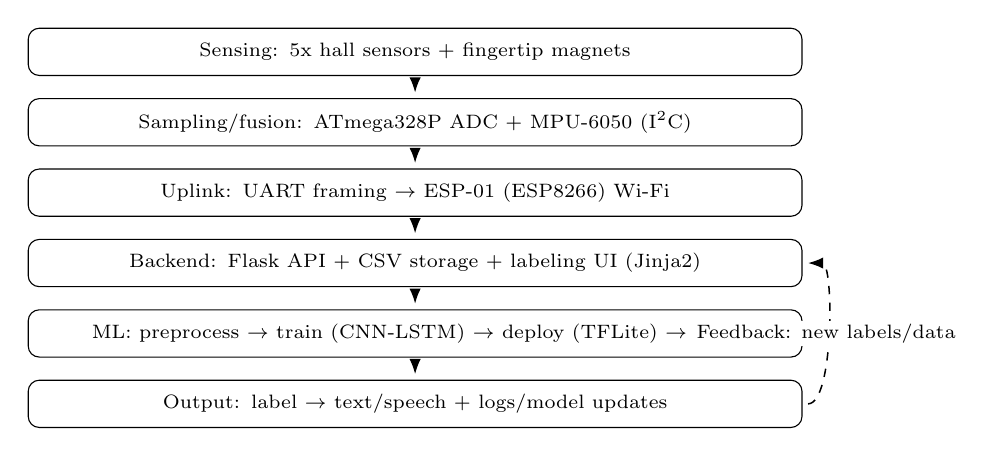
\begin{tikzpicture}[font=\scriptsize, node distance=2.8mm, every node/.style={inner sep=1.8pt}]
        \tikzset{
            box/.style={draw, rounded corners, align=center, text width=0.80\linewidth, minimum height=6.0mm},
            arr/.style={-Latex, line width=0.55pt, shorten <=2pt, shorten >=2pt}
        }

        \node[box] (sens) {Sensing: 5x hall sensors + fingertip magnets};
        \node[box, below=of sens] (mcu) {Sampling/fusion: ATmega328P ADC + MPU-6050 (I\textsuperscript{2}C)};
        \node[box, below=of mcu] (link) {Uplink: UART framing $\rightarrow$ ESP-01 (ESP8266) Wi-Fi};
        \node[box, below=of link] (backend) {Backend: Flask API + CSV storage + labeling UI (Jinja2)};
        \node[box, below=of backend] (ml) {ML: preprocess $\rightarrow$ train (CNN-LSTM) $\rightarrow$ deploy (TFLite) $\rightarrow$ infer};
        \node[box, below=of ml] (out) {Output: label $\rightarrow$ text/speech + logs/model updates};

        \draw[arr] (sens) -- (mcu);
        \draw[arr] (mcu) -- (link);
        \draw[arr] (link) -- (backend);
        \draw[arr] (backend) -- (ml);
        \draw[arr] (ml) -- (out);

        % Feedback loop kept inside the column-width frame (small right-side curve).
        \draw[arr, dashed]
            (out.east) .. controls +(4mm,0mm) and +(4mm,0mm) ..
            node[midway, fill=white, inner sep=1pt]{Feedback: new labels/data}
            (backend.east);
    \end{tikzpicture}
    \end{minipage}%
    }%
    \caption{System-level block diagram illustrating SSLG's hardware-software interactions.}
    \label{fig:block}
\end{figure}

\vspace{-2pt}
\noindent\textbf{D. Circuit Diagram.}
\FigLink{fig:circuit} provides the complete circuit diagram used for the prototype implementation. It covers the power tree (battery, charging, and regulation), sensor interfaces, microcontroller wiring, and the wireless communication interface.

The schematic highlights two practical needs in wearable hardware: stable power rails and clean sensor signals. The boost/buck stages provide 5 V and 3.3 V supplies for the mixed-voltage modules, while local decoupling reduces voltage dips during Wi-Fi transmit bursts. Sensor lines are routed to the ATmega328P ADC and I\textsuperscript{2}C pins, and the UART link connects the ATmega328P to the ESP-01 for wireless uplink. For quick verification during testing, the power tree should be checked first (battery to rails), followed by the sensor inputs, and finally the serial communication lines.

\begin{figure*}[!b]
    \centering
    % KiCad export with trim to enlarge the core drawing (preferred). If the PDF is
    % missing, a PNG export can be used as a fallback.
    \IfFileExists{KICAD_SL_PDF.pdf}{%
        \FrameBoxText{%
        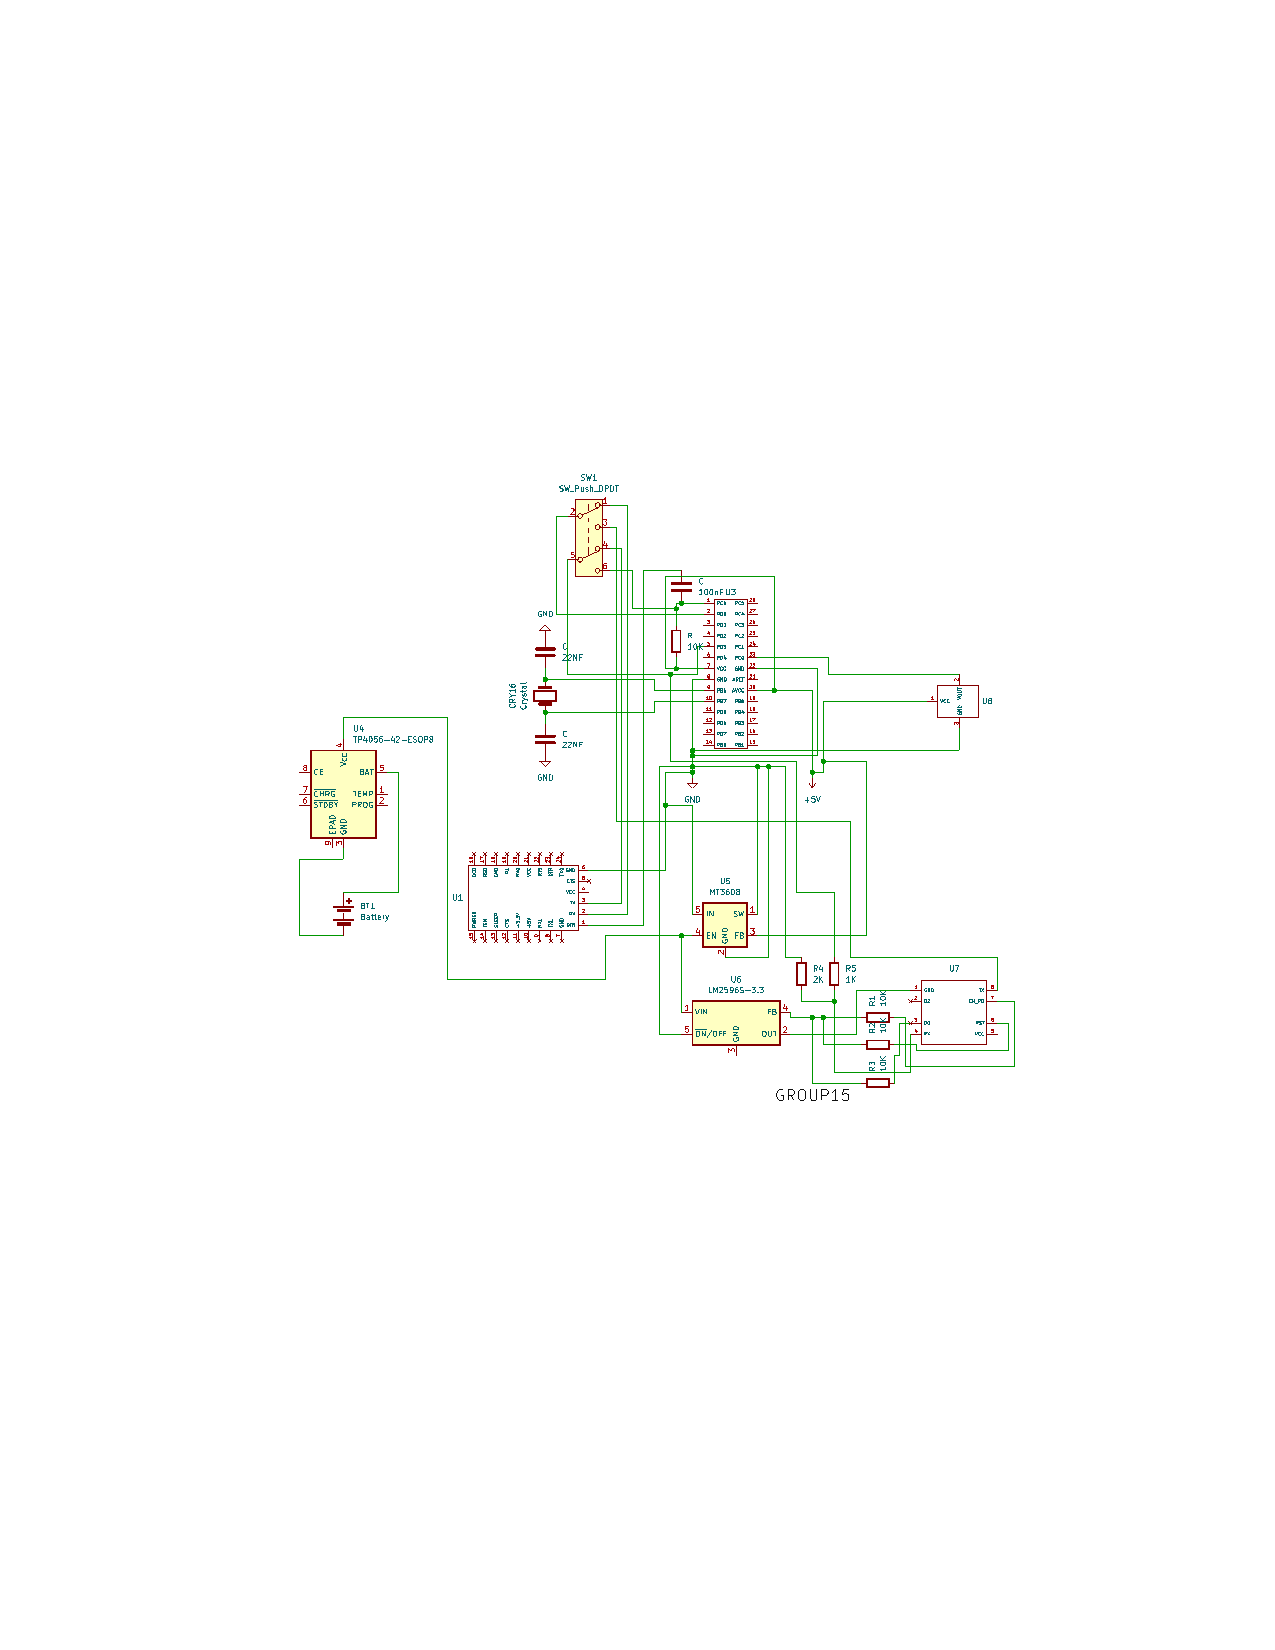
\includegraphics[page=1,width=\linewidth,height=0.82\textheight,keepaspectratio,trim=40mm 85mm 40mm 80mm,clip]{KICAD_SL_PDF.pdf}%
        }%
    }{%
        \IfFileExists{sslg_full_circuit.png}{%
            \FrameBoxText{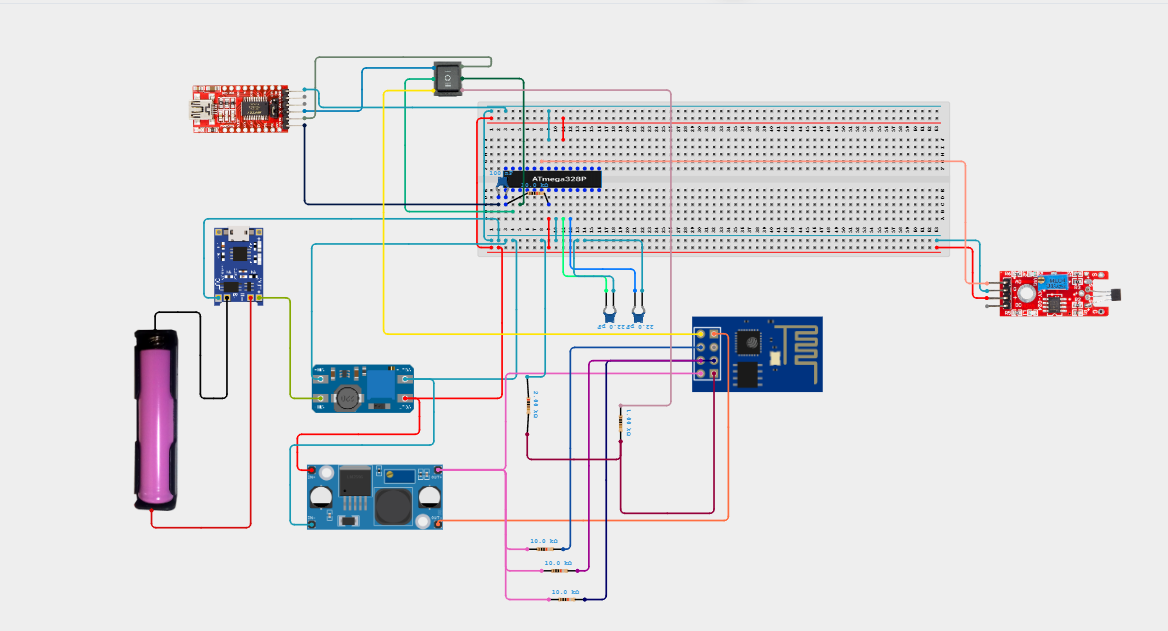
\includegraphics[width=\linewidth,keepaspectratio]{sslg_full_circuit.png}}%
        }{%
            \FrameBoxText{\parbox{0.95\linewidth}{\centering \textbf{Missing circuit diagram}\\Add \texttt{KICAD\_SL\_PDF.pdf} (preferred) or \texttt{sslg\_full\_circuit.png}.}}%
        }%
    }%
    \caption{Complete circuit schematic of the SSLG system (KiCad export).}
    \label{fig:circuit}
\end{figure*}

\noindent\textbf{How to read the schematic:} Start with the power path (battery $\rightarrow$ TP4056 $\rightarrow$ 5 V boost and 3.3 V buck). Then follow the sensor connections into the ATmega328P ADC and I\textsuperscript{2}C pins, and finally verify the UART connections between the ATmega328P and ESP-01.
\FloatBarrier

\section{Implementation}
\subsection{Data Collection \& Preprocessing}
Volunteers perform 20 ISL gestures. Each session generates labeled CSV rows stored on the Flask server. Preprocessing normalizes each sensor channel and applies noise filtering as shown earlier. Oversampling balances underrepresented classes, ensuring the dataset has roughly 1,000 records per gesture. Table~\ref{tab:dataset} summarizes the dataset.

\subsection{Calibration Procedure}
Before each session, SSLG applies a short calibration routine to reduce inter-session variance. The user holds an open palm ``neutral'' pose for a fixed time window (e.g., 3 seconds). For each hall channel $i$, we compute a baseline $b_i$ (mean value over the window) and store it in EEPROM or flash configuration. Subsequent readings use $\Delta_i = x_i - b_i$ so that the classifier learns relative deflection rather than absolute ADC readings. Similar baseline subtraction is applied to accelerometer channels to reduce bias.

\subsection{Windowing and Feature Formation}
Gesture classification benefits from treating sensor streams as short windows rather than single samples. SSLG therefore segments data into windows of $W$ samples (e.g., 25--50) with overlap $O$ (e.g., 50\%). Each window becomes a tensor of shape $W \times C$ where $C$ includes 5 hall channels and 6 IMU channels. This format is compatible with 1D convolution and recurrent layers and reduces sensitivity to small timing differences between signers.

\begin{table}[htbp]
    \centering
    \caption{Dataset Snapshot (Example Structure)}
    \label{tab:dataset}
    \begin{tabularx}{\columnwidth}{@{}lclX@{}}
        \toprule
        Gesture & Samples & Key Feature \\
        \midrule
        Hello & 1024 & Strong hall readings on thumb \\
        Thank you & 980 & Subtle wrist tilt + magnet shift \\
        Yes & 1012 & Combined flexed fingers \\
        No & 995 & Accelerometer variance \\
        Others (16 gestures) & 16\,000 & Balanced mix \\
        \bottomrule
    \end{tabularx}
\end{table}

\subsection{ML Pipeline}
We use a CNN-LSTM model: two 1D convolutional layers (kernel=3, filters=32/64), followed by an LSTM layer with 128 units and a dense softmax head over 20 classes. Dropout of 0.4 reduces overfitting, and AMSGrad trains with categorical cross-entropy. TensorFlow is used for training and for converting the model to TensorFlow Lite (8-bit quantization) for faster inference\cite{tensorflow}.

\begin{figure}[htbp]
    \centering
    % If you prefer an external ML architecture figure, use:
    % \includegraphics[width=\linewidth]{figures/sslg_ml_pipeline.png}
    \FrameBoxCol{%
    \vspace*{2mm}%
    \begin{minipage}{0.94\linewidth}
    \centering
    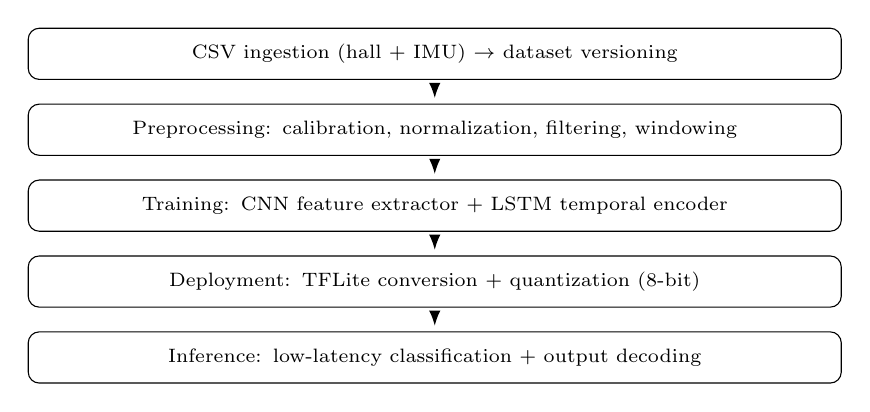
\begin{tikzpicture}[font=\scriptsize, node distance=3mm, every node/.style={inner sep=2pt}]
        \tikzset{
            p/.style={draw, rounded corners, align=center, text width=0.84\linewidth, minimum height=6.5mm},
            arr/.style={-Latex, line width=0.55pt, shorten <=2pt, shorten >=2pt}
        }
        \node[p] (ing) {CSV ingestion (hall + IMU) $\rightarrow$ dataset versioning};
        \node[p, below=of ing] (prep) {Preprocessing: calibration, normalization, filtering, windowing};
        \node[p, below=of prep] (train) {Training: CNN feature extractor + LSTM temporal encoder};
        \node[p, below=of train] (tfl) {Deployment: TFLite conversion + quantization (8-bit)};
        \node[p, below=of tfl] (inf) {Inference: low-latency classification + output decoding};
        \draw[arr] (ing) -- (prep);
        \draw[arr] (prep) -- (train);
        \draw[arr] (train) -- (tfl);
        \draw[arr] (tfl) -- (inf);
    \end{tikzpicture}
    \end{minipage}%
    \vspace*{2mm}%
    }%
    \caption{High-level machine learning pipeline for SSLG.}
    \label{fig:mlflow}
\end{figure}

\subsection{Firmware Processing Flow}
\begin{figure}[htbp]
    \centering
    % If you prefer an external firmware flowchart, use:
    % \includegraphics[width=\linewidth]{figures/sslg_firmware_flow.png}
    \FrameBoxCol{%
    \vspace*{2mm}%
    \begin{minipage}{0.94\linewidth}
    \centering
    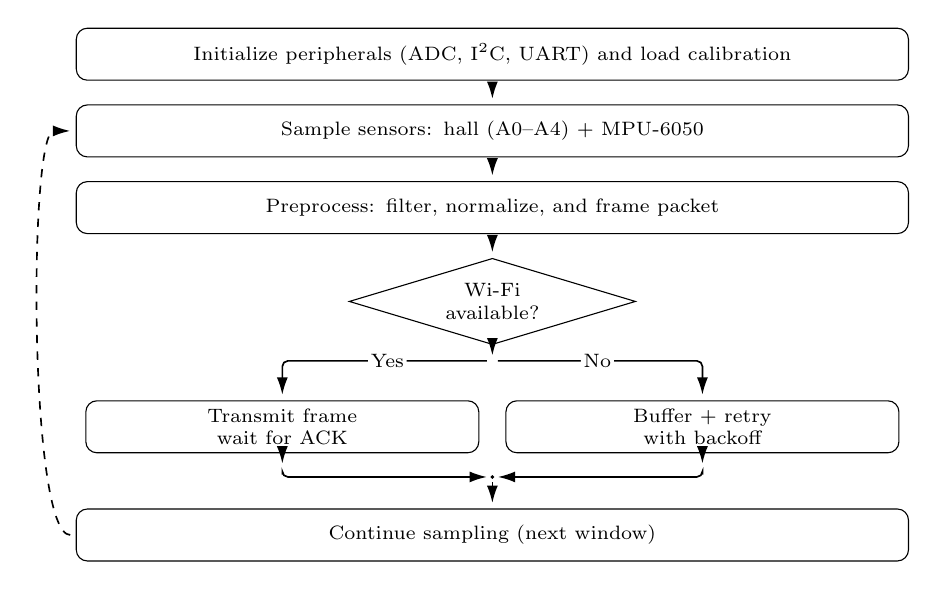
\begin{tikzpicture}[font=\scriptsize, every node/.style={inner sep=2pt}]
        \tikzset{
            st/.style={draw, rounded corners, align=center, text width=0.86\linewidth, minimum height=6.6mm},
            br/.style={draw, rounded corners, align=center, text width=0.40\linewidth, minimum height=6.6mm},
            dec/.style={draw, diamond, aspect=2.2, align=center, inner sep=1pt, minimum width=0.30\linewidth, minimum height=7.6mm},
            arr/.style={-{Latex[length=2.2mm,width=1.4mm]}, line width=0.6pt, shorten <=2pt, shorten >=2pt, rounded corners=2pt}
        }

        % Main vertical flow
        \node[st] (init) {Initialize peripherals (ADC, I\textsuperscript{2}C, UART) and load calibration};
        \node[st, below=3mm of init] (sample) {Sample sensors: hall (A0--A4) + MPU-6050};
        \node[st, below=3mm of sample] (prep) {Preprocess: filter, normalize, and frame packet};
        \node[dec, below=3mm of prep] (wifiok) {Wi-Fi\\available?};

        % Branches (kept strictly inside the frame using symmetric x-shifts)
        \node[br, below=7mm of wifiok, xshift=-0.22\linewidth] (tx) {Transmit frame\\wait for ACK};
        \node[br, below=7mm of wifiok, xshift=0.22\linewidth] (buf) {Buffer + retry\\with backoff};

        % Merge and continue
        \coordinate (mid) at ($(tx.south)!0.5!(buf.south)$);
        \node[st, below=7mm of mid] (next) {Continue sampling (next window)};
        \coordinate (merge) at ($(tx.south)!0.5!(buf.south) + (0,-3mm)$);

        \draw[arr] (init) -- (sample);
        \draw[arr] (sample) -- (prep);
        \draw[arr] (prep) -- (wifiok);

        % Cleaner branch routing: first drop down, then route to each branch.
        \coordinate (wifidrop) at ($(wifiok.south)+(0,-2mm)$);
        \draw[arr] (wifiok.south) -- (wifidrop);
        \draw[arr] (wifidrop) -| node[pos=0.25, fill=white, inner sep=1pt]{Yes} (tx.north);
        \draw[arr] (wifidrop) -| node[pos=0.25, fill=white, inner sep=1pt]{No} (buf.north);

        % Merge with a visible junction.
        \coordinate (txdrop) at ($(tx.south)+(0,-2mm)$);
        \coordinate (bufdrop) at ($(buf.south)+(0,-2mm)$);
        \draw[arr] (tx.south) -- (txdrop);
        \draw[arr] (buf.south) -- (bufdrop);
        \draw[arr] (txdrop) |- (merge);
        \draw[arr] (bufdrop) |- (merge);
        \fill (merge) circle (0.7pt);
        \draw[arr] (merge) -- (next.north);

        % Compact loop kept inside the frame.
        \draw[arr, dashed] (next.west) .. controls +(-6mm,0mm) and +(-6mm,0mm) .. (sample.west);
    \end{tikzpicture}
    \end{minipage}%
    \vspace*{2mm}%
    }%
    \caption{Firmware-level acquisition and transmission flow on ATmega328P.}
    \label{fig:firmware}
\end{figure}

\subsection{Backend \& UI}
The Flask backend provides endpoints for data ingestion, labeling, training, and inference\cite{flask}. The Jinja2 UI shows the live sensor stream and lets the user confirm gesture labels during data collection. A retraining option is provided so the model can be updated after new samples are added.

\subsection{Backend Workflow and Data Management}
The backend follows a simple, repeatable flow: (i) ingest packets and store decoded CSV rows, (ii) assign a gesture label and basic session details, (iii) preprocess and build the training dataset, (iv) train and save the model with basic evaluation logs, and (v) run inference and return the predicted label and confidence. Keeping these steps separate makes it easier to debug the system and to understand which data and model version produced a given result.

\begin{figure}[htbp]
    \centering
    % \includegraphics[width=\linewidth]{figures/backend_workflow.png}
    \FrameBoxCol{%
    \vspace*{2mm}%
    \begin{minipage}{0.94\linewidth}
    \centering
    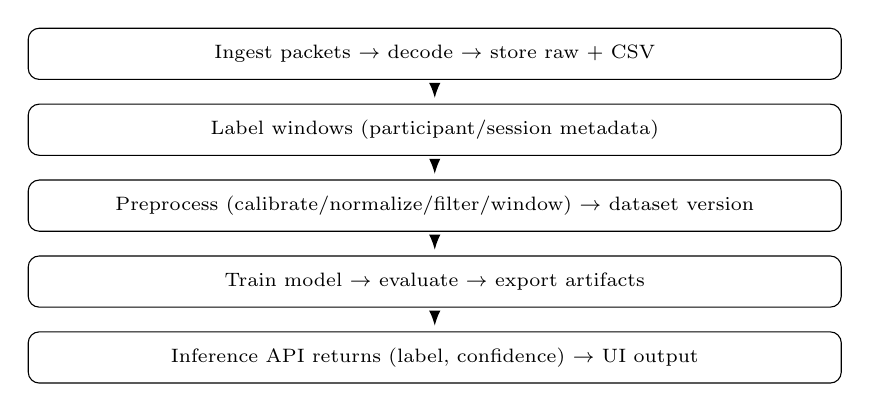
\begin{tikzpicture}[font=\scriptsize, node distance=3mm, every node/.style={inner sep=2pt}]
        \tikzset{
            p/.style={draw, rounded corners, align=center, text width=0.84\linewidth, minimum height=6.5mm},
            arr/.style={-Latex, line width=0.55pt, shorten <=2pt, shorten >=2pt}
        }
        \node[p] (ing) {Ingest packets $\rightarrow$ decode $\rightarrow$ store raw + CSV};
        \node[p, below=of ing] (lab) {Label windows (participant/session metadata)};
        \node[p, below=of lab] (prep) {Preprocess (calibrate/normalize/filter/window) $\rightarrow$ dataset version};
        \node[p, below=of prep] (train) {Train model $\rightarrow$ evaluate $\rightarrow$ export artifacts};
        \node[p, below=of train] (infer) {Inference API returns (label, confidence) $\rightarrow$ UI output};
        \draw[arr] (ing) -- (lab);
        \draw[arr] (lab) -- (prep);
        \draw[arr] (prep) -- (train);
        \draw[arr] (train) -- (infer);
    \end{tikzpicture}
    \end{minipage}%
    \vspace*{2mm}%
    }%
    \caption{Backend workflow for data collection, labeling, dataset versioning, training, and inference.}
    \label{fig:backendflow}
\end{figure}

\subsection{CSV Schema (Suggested)}
To keep the dataset easy to use, the stored CSV should follow a consistent schema. Table~\ref{tab:csvschema} shows a recommended column layout. If storage is limited, derived fields (such as normalized signals) can be computed during training instead of storing them.

\begin{table}[htbp]
    \centering
    \caption{Suggested CSV Column Schema}
    \label{tab:csvschema}
    \begin{tabularx}{\columnwidth}{@{}lX@{}}
        \toprule
        Column & Description \\
        \midrule
        ts\_ms & Timestamp (ms) \\
        hall0..hall4 & Raw hall ADC channels \\
        ax, ay, az & Accelerometer axes \\
        gx, gy, gz & Gyroscope axes \\
        label\_id & Gesture ID (integer) \\
        label\_name & Gesture name (string) \\
        participant\_id & Anonymous participant ID \\
        session\_id & Session identifier \\
        \bottomrule
    \end{tabularx}
\end{table}

\subsection{Flask API Endpoints (Suggested)}
The following endpoint structure keeps collection, labeling, training, and inference decoupled and testable:
\begin{itemize}[noitemsep]
    \item \texttt{POST /api/ingest}: receive packets/JSON and store decoded rows.
    \item \texttt{POST /api/label}: assign/confirm labels for a buffered window.
    \item \texttt{POST /api/train}: train a model on the selected dataset version.
    \item \texttt{POST /api/infer}: return predicted label and confidence for a new window.
    \item \texttt{GET /ui/collect}, \texttt{/ui/label}, \texttt{/ui/infer}: Jinja2 pages for workflow.
\end{itemize}

\subsection{Sample JSON Packet Received at Backend}
Listing~\ref{lst:json_packet} shows an example JSON payload received by the backend ingestion endpoint. The ESP-01 can either forward decoded fields as JSON (recommended for readability during development) or forward a binary frame that the server decodes into the same JSON structure.

\begin{lstlisting}[style=sslgcode, caption={Sample JSON packet received at the backend (\texttt{POST /api/ingest}).}, label={lst:json_packet}]
{
  "device_id": "SSLG-01",
  "fw_ver": "1.0.0",
  "ts_ms": 128734,
  "mode": "collect",
  "hall_adc": [512, 498, 530, 475, 510],
  "imu_lsb": {
    "ax": -120, "ay": 340, "az": 16320,
    "gx": 12, "gy": -8, "gz": 3
  },
  "label_id": 5,
  "label_name": "THANK_YOU",
  "rssi_dbm": -55
}
\end{lstlisting}

\subsection{Sample Backend Code (Flask)}
Listing~\ref{lst:flask_ingest} shows a minimal ingestion endpoint and an inference endpoint skeleton. In a full implementation, these handlers should validate input fields and log errors to simplify debugging.

\begin{lstlisting}[style=sslgcode, caption={Minimal Flask endpoints for ingestion and inference (skeleton).}, label={lst:flask_ingest}, language=Python]
from flask import Flask, request, jsonify
import time

app = Flask(__name__)

@app.post("/api/ingest")
def ingest():
    payload = request.get_json(force=True)
    # Expected: {"ts_ms":..., "hall":[...], "imu":[...], "label_id":...}
    # TODO: validate + store to CSV/database
    return jsonify({"ok": True, "received_at": int(time.time() * 1000)})

@app.post("/api/infer")
def infer():
    window = request.get_json(force=True)
    # TODO: preprocess window -> model.predict -> decode label
    return jsonify({"label_id": -1, "label_name": "TBD", "confidence": 0.0})
\end{lstlisting}

\subsection{Sample Firmware Code (ATmega328P)}
Listing~\ref{lst:firmware_pack} illustrates how firmware can sample analog hall channels, read IMU values, and pack a simple UART frame. The final build should include a checksum and a protocol version byte as described in Table~\ref{tab:packet}.

\begin{lstlisting}[style=sslgcode, caption={ATmega328P sampling and UART packet framing (illustrative).}, label={lst:firmware_pack}, language=C]
// Pseudocode-style C/Arduino snippet
uint16_t hall[5];
int16_t imu[6];

void sample_hall() {
  for (int i = 0; i < 5; i++) hall[i] = analogRead(A0 + i);
}

void send_frame() {
  Serial.write(0xAA);        // preamble
  Serial.write(0x01);        // version
  uint16_t ts = millis();    // timestamp (wraps)
  Serial.write((uint8_t)(ts & 0xFF));
  Serial.write((uint8_t)(ts >> 8));
  for (int i = 0; i < 5; i++) { // hall: little-endian
    Serial.write((uint8_t)(hall[i] & 0xFF));
    Serial.write((uint8_t)(hall[i] >> 8));
  }
  for (int i = 0; i < 6; i++) { // imu: little-endian
    Serial.write((uint8_t)(imu[i] & 0xFF));
    Serial.write((uint8_t)(imu[i] >> 8));
  }
  // TODO: checksum byte
}
\end{lstlisting}

\subsection{Power Budget Estimation}
Battery life depends on Wi-Fi burst currents and converter losses. A conservative estimate assumes the ESP8266 draws bursts of 200--300\,mA during transmission while the ATmega328P and sensors operate at lower steady currents. For reporting, record (i) average current during idle collection, (ii) average current during inference bursts, and (iii) end-to-end runtime until the battery reaches a safe cutoff voltage. This power characterization is crucial for a wearable system and should be reported alongside accuracy and latency.

\section{Results and Discussion}
\subsection{Experimental Setup}
Tests are planned in a university laboratory environment. Each gesture will be repeated across multiple trials and participants to ensure coverage of signer variability. Battery-powered operation will be used to characterize autonomy under realistic usage patterns.

The backend server can run on a standard laptop (e.g., Intel Core i5-class CPU, 8\,GB RAM) with Python and Flask. During evaluation, Flask endpoints should operate over a dedicated 2.4\,GHz Wi-Fi access point to reduce interference. Round-trip latency will be logged from sensor packet capture to the inference response, and each session will start with calibration to a neutral open palm reference.

\subsection{Performance Evaluation}
The evaluation will report standard classification metrics (accuracy, precision, recall, F1) and latency (sensor-to-output time). Since integrated prototype testing is pending, Table~\ref{tab:metrics} provides a structured format to record results.

\begin{table}[htbp]
    \centering
    \caption{Final Results Reporting Template (Expected Values)}
    \label{tab:metrics}
    \begin{tabularx}{\columnwidth}{@{}lX@{}}
        \toprule
        Metric & Expected value (to be validated experimentally) \\
        \midrule
        Accuracy (\%) & 92--95 \\
        Precision & 0.92 \\
        Recall & 0.91 \\
        F1-score & 0.91--0.93 \\
        Avg. end-to-end latency (ms) & 220--320 \\
        Peak end-to-end latency (ms) & 450--650 \\
        Battery autonomy (hours) & 3--5 \\
        \bottomrule
    \end{tabularx}
\end{table}

\begin{table}[htbp]
    \centering
    \caption{Qualitative Comparison of Common Approaches}
    \label{tab:comparison}
    \begin{tabularx}{\columnwidth}{@{}lXX@{}}
        \toprule
        Approach & Strengths & Limitations \\
        \midrule
        Camera-based & No wearable hardware; rich features & Occlusion; lighting; compute cost\cite{mitra} \\
        Flex-sensor glove & Low compute; direct finger bend & Mechanical fatigue; drift; nonlinearity \\
        Hall-sensor glove (SSLG) & More durable sensing; portable; low cost & Magnet placement sensitivity; calibration \\
        \bottomrule
    \end{tabularx}
\end{table}

\subsection{Discussion}
Hall sensors reduce mechanical wear compared to flex-based approaches and can give stable readings when magnet placement is consistent. On the software side, the Flask+Jinja2 workflow makes it easy to collect data, label it, and retrain the model as needed. The main practical issues are magnet placement changes during use, repeatable calibration across users, and occasional packet loss on Wi-Fi. When final testing is completed, the results section should include a confusion matrix and training curves, along with accuracy and latency numbers.

\section{Conclusion}
SSLG combines a hall-sensor glove with an ATmega328P sampling layer and a Flask-based backend to translate ISL gestures into text and speech. The key idea is to use hall sensors and magnets for more stable sensing than flex sensors, and to keep model training and inference on the backend so the system can be updated as new data is collected. This paper documented the hardware choices, the software workflow, and the evaluation plan. Future work will complete full prototype testing, expand the dataset across more users, and reduce latency with further optimizations.

\section{Future Scope}
Future work includes completing the integrated glove prototype, collecting data from more users in real settings, improving calibration and drift handling, and exploring offline inference to reduce dependence on network connectivity.

\section*{Acknowledgment}
The authors thank the Department of Electronics and Communication Engineering, Vidyavardhini's College of Engineering \& Technology, for providing facilities and guidance for this project.

\begin{thebibliography}{99}
\bibitem{mitra} S. Mitra and T. Acharya, ``Gesture recognition: A survey,'' \textit{IEEE Trans. Syst., Man, Cybern. Part C}, vol. 37, no. 3, pp. 311--324, May 2007. [Online]. Available: \url{https://ieeexplore.ieee.org/document/4270516}
\bibitem{tensorflow} TensorFlow Lite, ``TensorFlow Lite guide,'' 2024. [Online]. Available: \url{https://www.tensorflow.org/lite}
\bibitem{atmega328p} Microchip Technology, ``ATmega328P/328PB datasheet,'' 2016. [Online]. Available: \url{https://ww1.microchip.com/downloads/en/DeviceDoc/Atmel-42735-8-bit-AVR-Microcontroller-ATmega328-328P_Datasheet.pdf}
\bibitem{ft232rl} FTDI, ``FT232R USB UART IC,'' [Online]. Available: \url{https://ftdichip.com/products/ft232rl/}
\bibitem{tp4056} ``TP4056 Li-ion battery charger IC datasheet,'' [Online]. Available: \url{https://www.alldatasheet.com/datasheet-pdf/pdf/1132405/ETC2/TP4056.html}
\bibitem{battery18650} ``18650 battery overview,'' [Online]. Available: \url{https://en.wikipedia.org/wiki/18650_battery}
\bibitem{mt3608} ``MT3608 step-up converter IC datasheet,'' [Online]. Available: \url{https://www.alldatasheet.com/datasheet-pdf/pdf/1131964/ETC2/MT3608.html}
\bibitem{lm2596} Texas Instruments, ``LM2596 SIMPLE SWITCHER power converter datasheet,'' [Online]. Available: \url{https://www.ti.com/lit/ds/symlink/lm2596.pdf}
\bibitem{esp8266} Espressif Systems, ``ESP8266EX datasheet,'' 2019. [Online]. Available: \url{https://www.espressif.com/sites/default/files/documentation/0a-esp8266ex_datasheet_en.pdf}
\bibitem{ss49e} Honeywell, ``SS49E linear Hall-effect sensor datasheet,'' [Online]. Available: \url{https://www.mouser.com/datasheet/2/187/SS49E-1122400.pdf}
\bibitem{mpu6050} TDK InvenSense, ``MPU-6050 product specification,'' 2015. [Online]. Available: \url{https://invensense.tdk.com/wp-content/uploads/2015/02/MPU-6000-Datasheet1.pdf}
\bibitem{flask} Pallets Projects, ``Flask documentation,'' 2024. [Online]. Available: \url{https://flask.palletsprojects.com/en/2.2.x/}
\end{thebibliography}

\end{document}
